\documentclass[10pt]{beamer}

\usepackage[english]{babel}

\usepackage{lmodern}

\title{class}
\begin{document}
\section{The incomprehensible equations of Navier Stokes}
\begin{frame}
\textbf{definition}
Navier-Stokes equations are a system of nonlinear partial differential equations that describe the movement of fluids in a continuous medium.

\textbf{Reynolds number}
We will write the Navier-Stokes equation using dimensionless combinations (which
will be noted by premiums) of the different sizes involved. Let L and U be the scales
respective size and flow velocity, we have

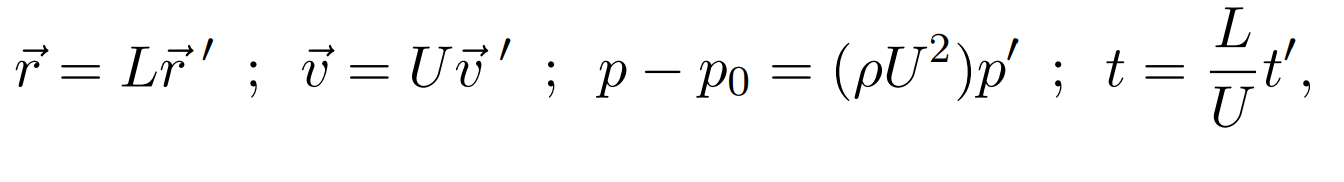
\includegraphics[scale=0.5]{images/equa1.png}
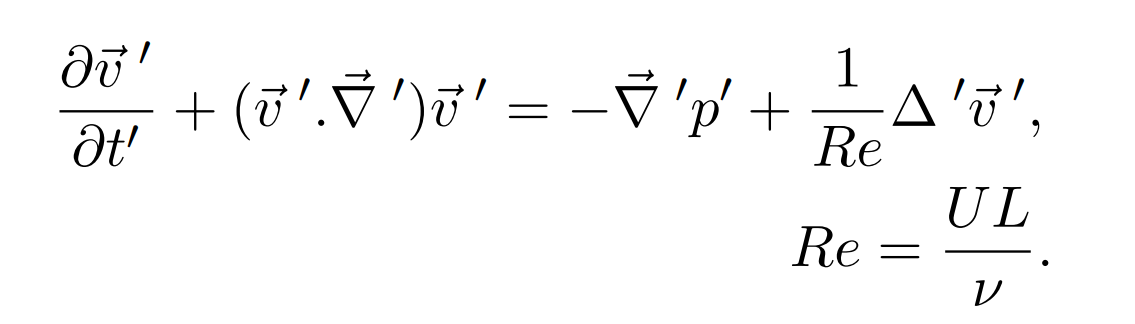
\includegraphics[scale=0.5]{images/equa2.png}
\begin{equation}

\end{equation}

There appears a dimensionless number, Re which is a combination of L, U and ν: the number of
Reynolds. It weighs the term viscous diffusion against the other terms in the equation.
We recognize the two characteristic times necessary to transport the momentum
over a length L by diffusion and by convection. Transportation will be the shortest time
thus dominating the Reynolds number is the relationship between convective and diffusive effects:
\frac{effet convectif}{effet diffusif}

It is also often useful to understand the Reynolds number as the relationship between the terms
of inertia and viscous forces of the Navier-Stokes equation

\frac{forces inertielles}{forces visqueuses}

\end{frame}

\end{document}